% Options for packages loaded elsewhere
% Options for packages loaded elsewhere
\PassOptionsToPackage{unicode}{hyperref}
\PassOptionsToPackage{hyphens}{url}
\PassOptionsToPackage{dvipsnames,svgnames,x11names}{xcolor}
%
\documentclass[
  authoryear,
  review,
  3p]{elsarticle}
\usepackage{xcolor}
\usepackage{amsmath,amssymb}
\setcounter{secnumdepth}{5}
\usepackage{iftex}
\ifPDFTeX
  \usepackage[T1]{fontenc}
  \usepackage[utf8]{inputenc}
  \usepackage{textcomp} % provide euro and other symbols
\else % if luatex or xetex
  \usepackage{unicode-math} % this also loads fontspec
  \defaultfontfeatures{Scale=MatchLowercase}
  \defaultfontfeatures[\rmfamily]{Ligatures=TeX,Scale=1}
\fi
\usepackage{lmodern}
\ifPDFTeX\else
  % xetex/luatex font selection
\fi
% Use upquote if available, for straight quotes in verbatim environments
\IfFileExists{upquote.sty}{\usepackage{upquote}}{}
\IfFileExists{microtype.sty}{% use microtype if available
  \usepackage[]{microtype}
  \UseMicrotypeSet[protrusion]{basicmath} % disable protrusion for tt fonts
}{}
\makeatletter
\@ifundefined{KOMAClassName}{% if non-KOMA class
  \IfFileExists{parskip.sty}{%
    \usepackage{parskip}
  }{% else
    \setlength{\parindent}{0pt}
    \setlength{\parskip}{6pt plus 2pt minus 1pt}}
}{% if KOMA class
  \KOMAoptions{parskip=half}}
\makeatother
% Make \paragraph and \subparagraph free-standing
\makeatletter
\ifx\paragraph\undefined\else
  \let\oldparagraph\paragraph
  \renewcommand{\paragraph}{
    \@ifstar
      \xxxParagraphStar
      \xxxParagraphNoStar
  }
  \newcommand{\xxxParagraphStar}[1]{\oldparagraph*{#1}\mbox{}}
  \newcommand{\xxxParagraphNoStar}[1]{\oldparagraph{#1}\mbox{}}
\fi
\ifx\subparagraph\undefined\else
  \let\oldsubparagraph\subparagraph
  \renewcommand{\subparagraph}{
    \@ifstar
      \xxxSubParagraphStar
      \xxxSubParagraphNoStar
  }
  \newcommand{\xxxSubParagraphStar}[1]{\oldsubparagraph*{#1}\mbox{}}
  \newcommand{\xxxSubParagraphNoStar}[1]{\oldsubparagraph{#1}\mbox{}}
\fi
\makeatother

\usepackage{color}
\usepackage{fancyvrb}
\newcommand{\VerbBar}{|}
\newcommand{\VERB}{\Verb[commandchars=\\\{\}]}
\DefineVerbatimEnvironment{Highlighting}{Verbatim}{commandchars=\\\{\}}
% Add ',fontsize=\small' for more characters per line
\usepackage{framed}
\definecolor{shadecolor}{RGB}{241,243,245}
\newenvironment{Shaded}{\begin{snugshade}}{\end{snugshade}}
\newcommand{\AlertTok}[1]{\textcolor[rgb]{0.68,0.00,0.00}{#1}}
\newcommand{\AnnotationTok}[1]{\textcolor[rgb]{0.37,0.37,0.37}{#1}}
\newcommand{\AttributeTok}[1]{\textcolor[rgb]{0.40,0.45,0.13}{#1}}
\newcommand{\BaseNTok}[1]{\textcolor[rgb]{0.68,0.00,0.00}{#1}}
\newcommand{\BuiltInTok}[1]{\textcolor[rgb]{0.00,0.23,0.31}{#1}}
\newcommand{\CharTok}[1]{\textcolor[rgb]{0.13,0.47,0.30}{#1}}
\newcommand{\CommentTok}[1]{\textcolor[rgb]{0.37,0.37,0.37}{#1}}
\newcommand{\CommentVarTok}[1]{\textcolor[rgb]{0.37,0.37,0.37}{\textit{#1}}}
\newcommand{\ConstantTok}[1]{\textcolor[rgb]{0.56,0.35,0.01}{#1}}
\newcommand{\ControlFlowTok}[1]{\textcolor[rgb]{0.00,0.23,0.31}{\textbf{#1}}}
\newcommand{\DataTypeTok}[1]{\textcolor[rgb]{0.68,0.00,0.00}{#1}}
\newcommand{\DecValTok}[1]{\textcolor[rgb]{0.68,0.00,0.00}{#1}}
\newcommand{\DocumentationTok}[1]{\textcolor[rgb]{0.37,0.37,0.37}{\textit{#1}}}
\newcommand{\ErrorTok}[1]{\textcolor[rgb]{0.68,0.00,0.00}{#1}}
\newcommand{\ExtensionTok}[1]{\textcolor[rgb]{0.00,0.23,0.31}{#1}}
\newcommand{\FloatTok}[1]{\textcolor[rgb]{0.68,0.00,0.00}{#1}}
\newcommand{\FunctionTok}[1]{\textcolor[rgb]{0.28,0.35,0.67}{#1}}
\newcommand{\ImportTok}[1]{\textcolor[rgb]{0.00,0.46,0.62}{#1}}
\newcommand{\InformationTok}[1]{\textcolor[rgb]{0.37,0.37,0.37}{#1}}
\newcommand{\KeywordTok}[1]{\textcolor[rgb]{0.00,0.23,0.31}{\textbf{#1}}}
\newcommand{\NormalTok}[1]{\textcolor[rgb]{0.00,0.23,0.31}{#1}}
\newcommand{\OperatorTok}[1]{\textcolor[rgb]{0.37,0.37,0.37}{#1}}
\newcommand{\OtherTok}[1]{\textcolor[rgb]{0.00,0.23,0.31}{#1}}
\newcommand{\PreprocessorTok}[1]{\textcolor[rgb]{0.68,0.00,0.00}{#1}}
\newcommand{\RegionMarkerTok}[1]{\textcolor[rgb]{0.00,0.23,0.31}{#1}}
\newcommand{\SpecialCharTok}[1]{\textcolor[rgb]{0.37,0.37,0.37}{#1}}
\newcommand{\SpecialStringTok}[1]{\textcolor[rgb]{0.13,0.47,0.30}{#1}}
\newcommand{\StringTok}[1]{\textcolor[rgb]{0.13,0.47,0.30}{#1}}
\newcommand{\VariableTok}[1]{\textcolor[rgb]{0.07,0.07,0.07}{#1}}
\newcommand{\VerbatimStringTok}[1]{\textcolor[rgb]{0.13,0.47,0.30}{#1}}
\newcommand{\WarningTok}[1]{\textcolor[rgb]{0.37,0.37,0.37}{\textit{#1}}}

\usepackage{longtable,booktabs,array}
\usepackage{calc} % for calculating minipage widths
% Correct order of tables after \paragraph or \subparagraph
\usepackage{etoolbox}
\makeatletter
\patchcmd\longtable{\par}{\if@noskipsec\mbox{}\fi\par}{}{}
\makeatother
% Allow footnotes in longtable head/foot
\IfFileExists{footnotehyper.sty}{\usepackage{footnotehyper}}{\usepackage{footnote}}
\makesavenoteenv{longtable}
\usepackage{graphicx}
\makeatletter
\newsavebox\pandoc@box
\newcommand*\pandocbounded[1]{% scales image to fit in text height/width
  \sbox\pandoc@box{#1}%
  \Gscale@div\@tempa{\textheight}{\dimexpr\ht\pandoc@box+\dp\pandoc@box\relax}%
  \Gscale@div\@tempb{\linewidth}{\wd\pandoc@box}%
  \ifdim\@tempb\p@<\@tempa\p@\let\@tempa\@tempb\fi% select the smaller of both
  \ifdim\@tempa\p@<\p@\scalebox{\@tempa}{\usebox\pandoc@box}%
  \else\usebox{\pandoc@box}%
  \fi%
}
% Set default figure placement to htbp
\def\fps@figure{htbp}
\makeatother





\setlength{\emergencystretch}{3em} % prevent overfull lines

\providecommand{\tightlist}{%
  \setlength{\itemsep}{0pt}\setlength{\parskip}{0pt}}



 
\usepackage[]{natbib}
\bibliographystyle{elsarticle-harv}


\usepackage{booktabs}
\usepackage{longtable}
\usepackage{array}
\usepackage{multirow}
\usepackage{wrapfig}
\usepackage{float}
\usepackage{colortbl}
\usepackage{pdflscape}
\usepackage{tabu}
\usepackage{threeparttable}
\usepackage{threeparttablex}
\usepackage[normalem]{ulem}
\usepackage{makecell}
\usepackage{xcolor}
\usepackage{siunitx}

    \newcolumntype{d}{S[
      table-align-text-before=false,
      table-align-text-after=false,
      input-symbols={-,\*+()}
    ]}
  
\usepackage{tabularray}
\usepackage[normalem]{ulem}
\usepackage{graphicx}
\usepackage{rotating}
\UseTblrLibrary{siunitx}
\NewTableCommand{\tinytableDefineColor}[3]{\definecolor{#1}{#2}{#3}}
\newcommand{\tinytableTabularrayUnderline}[1]{\underline{#1}}
\newcommand{\tinytableTabularrayStrikeout}[1]{\sout{#1}}
\usepackage{xcolor}
\newcommand{\cw}[1]{\textcolor{orange}{#1}}
\newcommand{\Junyi}[1]{\textcolor{purple}{#1}}
\newcommand{\Ruth}[1]{\textcolor{teal}{#1}}
\newcommand{\Greg}[1]{\textcolor{blue}{#1}}
\newcommand{\Yongqi}[1]{\textcolor{violet}{#1}}
\newcommand{\Linda}[1]{\textcolor{pink}{#1}}
\renewcommand\thefootnote{\textcolor{orange}{\arabic{footnote}}}
\newcommand{\cwfn}[1]{\footnote{\textcolor{orange}{CW: #1}}}
\newcommand{\Junyifn}[1]{\footnote{\textcolor{purple}{Junyi: #1}}}
\usepackage{setspace}
\AtBeginEnvironment{tblr}{\begin{singlespacing}}
\AtEndEnvironment{tblr}{\end{singlespacing}}
\makeatletter
\@ifpackageloaded{caption}{}{\usepackage{caption}}
\AtBeginDocument{%
\ifdefined\contentsname
  \renewcommand*\contentsname{Table of contents}
\else
  \newcommand\contentsname{Table of contents}
\fi
\ifdefined\listfigurename
  \renewcommand*\listfigurename{List of Figures}
\else
  \newcommand\listfigurename{List of Figures}
\fi
\ifdefined\listtablename
  \renewcommand*\listtablename{List of Tables}
\else
  \newcommand\listtablename{List of Tables}
\fi
\ifdefined\figurename
  \renewcommand*\figurename{Figure}
\else
  \newcommand\figurename{Figure}
\fi
\ifdefined\tablename
  \renewcommand*\tablename{Table}
\else
  \newcommand\tablename{Table}
\fi
}
\@ifpackageloaded{float}{}{\usepackage{float}}
\floatstyle{ruled}
\@ifundefined{c@chapter}{\newfloat{codelisting}{h}{lop}}{\newfloat{codelisting}{h}{lop}[chapter]}
\floatname{codelisting}{Listing}
\newcommand*\listoflistings{\listof{codelisting}{List of Listings}}
\makeatother
\makeatletter
\makeatother
\makeatletter
\@ifpackageloaded{caption}{}{\usepackage{caption}}
\@ifpackageloaded{subcaption}{}{\usepackage{subcaption}}
\makeatother
\journal{Transportation Research Part C: Emerging Technologies}
\usepackage{bookmark}
\IfFileExists{xurl.sty}{\usepackage{xurl}}{} % add URL line breaks if available
\urlstyle{same}
\hypersetup{
  pdftitle={Towards Accelerating Transportation Research: Measuring the Practice of Open Science},
  pdfauthor={Junyi Ji; Ruth Lu; Yongqin Dong; Liming Wang; Bahman Madadi; Silvia Varotto; Nicolas Saunier; Gregory S. Macfarlane; Mostafa Ameli; Cathy Wu},
  pdfkeywords={Open Science, Large Language Models},
  colorlinks=true,
  linkcolor={blue},
  filecolor={Maroon},
  citecolor={Blue},
  urlcolor={Blue},
  pdfcreator={LaTeX via pandoc}}


\setlength{\parindent}{6pt}
\begin{document}

\begin{frontmatter}
\title{Towards Accelerating Transportation Research: Measuring the
Practice of Open Science}
\author[]{Junyi Ji%
%
}

\author[]{Ruth Lu%
%
}

\author[]{Yongqin Dong%
%
}

\author[]{Liming Wang%
%
}

\author[]{Bahman Madadi%
%
}

\author[]{Silvia Varotto%
%
}

\author[]{Nicolas Saunier%
%
}

\author[1]{Gregory S. Macfarlane%
%
}

\author[]{Mostafa Ameli%
%
}

\author[2]{Cathy Wu%
\corref{cor1}%
}
 \ead{cathywu@mit.edu} 

\affiliation[1]{organization={Brigham Young University, Civil and
Construction Engineering},,postcodesep={}}
\affiliation[2]{organization={Massachusetts Institute of
Technology, Civil and Environmental Engineering},,postcodesep={}}

\cortext[cor1]{Corresponding author}










        
\begin{abstract}
This is the abstract. Lorem ipsum dolor sit amet, consectetur adipiscing
elit. Vestibulum augue turpis, dictum non malesuada a, volutpat eget
velit. Nam placerat turpis purus, eu tristique ex tincidunt et. Mauris
sed augue eget turpis ultrices tincidunt. Sed et mi in leo porta
egestas. Aliquam non laoreet velit. Nunc quis ex vitae eros aliquet
auctor nec ac libero. Duis laoreet sapien eu mi luctus, in bibendum leo
molestie. Sed hendrerit diam diam, ac dapibus nisl volutpat vitae.
Aliquam bibendum varius libero, eu efficitur justo rutrum at. Sed at
tempus elit.
\end{abstract}





\begin{keyword}
    Open Science \sep 
    Large Language Models
\end{keyword}
\end{frontmatter}
    

\section{Introduction}\label{intro}

I need a citation to keep from getting a latex error, so
\citet{nosek2015promoting} is a good one.

\section{Analysis}\label{analysis}

\subsection{Descriptive statistics and bivariate
tests}\label{descriptive-statistics-and-bivariate-tests}

The analysis dataset contains 10 480 papers that report quantitative
studies (\texttt{is\_quantitative\_study}) among the full-length
articles. Table~\ref{tbl-descriptives} provides descriptive statistics
for the dataset, organized by code availability. provides descriptive
statistics for these papers, organized by code availability. The dataset
contains 528 papers with code available, a little more than 0 \% of the
dataset. x In total, about 68.7\% of the papers cite available data, but
only 30.2\% of the papers include a data repository; the remaining 1\%
neither cite data nor include a repository.

\begin{table}

\caption{\label{tbl-descriptives}Descriptive Statistics of Data Set}

\centering{

\centering\centering
\resizebox{\ifdim\width>\linewidth\linewidth\else\width\fi}{!}{
\begin{tabular}[t]{llrrrr}
\toprule
\multicolumn{2}{c}{ } & \multicolumn{2}{c}{Code is not available (N=9952)} & \multicolumn{2}{c}{Code is available (N=528)} \\
\cmidrule(l{3pt}r{3pt}){3-4} \cmidrule(l{3pt}r{3pt}){5-6}
  &    & Mean & Std. Dev. & Mean & Std. Dev.\\
\midrule
Open science score &  & \num{2.2} & \num{0.6} & \num{3.4} & \num{1.1}\\
Age of paper [years] &  & \num{3.4} & \num{1.7} & \num{3.1} & \num{1.7}\\
N. tables in paper &  & \num{6.4} & \num{4.5} & \num{6.3} & \num{4.6}\\
N. figures in paper &  & \num{8.6} & \num{6.1} & \num{11.0} & \num{6.5}\\
N. references &  & \num{58.2} & \num{26.9} & \num{57.3} & \num{21.0}\\
N. authors &  & \num{3.8} & \num{1.7} & \num{3.8} & \num{1.7}\\
Times cited &  & \num{28.4} & \num{43.2} & \num{27.2} & \num{42.9}\\
Review time [days] &  & \num{254.3} & \num{148.9} & \num{268.6} & \num{141.4}\\
Page count &  & \num{18.4} & \num{6.3} & \num{19.8} & \num{6.6}\\
\midrule
 &  & N & Pct. & N & Pct.\\
\midrule\\
Open Access & Not open access & \num{7346} & \num{73.8} & \num{324} & \num{61.4}\\
 & Open access & \num{2606} & \num{26.2} & \num{204} & \num{38.6}\\
\midrule
Data availability & No repository or citation & \num{7063} & \num{71.0} & \num{139} & \num{26.3}\\
 & Data repository is available & \num{65} & \num{0.7} & \num{199} & \num{37.7}\\
 & Data is cited or linked & \num{2810} & \num{28.2} & \num{96} & \num{18.2}\\
 & Data repository and citation & \num{14} & \num{0.1} & \num{94} & \num{17.8}\\
\midrule
Journal & Interdisciplinary Perspectives & \num{945} & \num{9.5} & \num{36} & \num{6.8}\\
 & Part A: Policy and Practice & \num{1555} & \num{15.6} & \num{64} & \num{12.1}\\
 & Part B: Methodological & \num{771} & \num{7.7} & \num{67} & \num{12.7}\\
 & Part C: Emerging Technologies & \num{1797} & \num{18.1} & \num{212} & \num{40.2}\\
 & Part D: Transport and Environment & \num{1911} & \num{19.2} & \num{72} & \num{13.6}\\
 & Part E: Logistics and Transportation Review & \num{1534} & \num{15.4} & \num{41} & \num{7.8}\\
 & Part F: Traffic Psychology and Behaviour & \num{1439} & \num{14.5} & \num{36} & \num{6.8}\\
\midrule
Region of corr. author & Africa & \num{69} & \num{0.7} & \num{5} & \num{0.9}\\
 & Asia & \num{4398} & \num{44.2} & \num{118} & \num{22.3}\\
 & Europe & \num{2699} & \num{27.1} & \num{206} & \num{39.0}\\
 & North America & \num{2074} & \num{20.8} & \num{156} & \num{29.5}\\
 & Oceania & \num{521} & \num{5.2} & \num{27} & \num{5.1}\\
 & South America & \num{191} & \num{1.9} & \num{16} & \num{3.0}\\
\midrule
Availability statement & Availability statement is not present & \num{7062} & \num{71.0} & \num{139} & \num{26.3}\\
 & Availability statement is present & \num{2890} & \num{29.0} & \num{389} & \num{73.7}\\
\midrule
Paper topic & Air \& Freight Logistics & \num{77} & \num{0.8} & \num{2} & \num{0.4}\\
 & Automated Driving \& Human Factors & \num{957} & \num{9.6} & \num{34} & \num{6.4}\\
 & COVID-19 Impact on Travel \& Activities & \num{434} & \num{4.4} & \num{17} & \num{3.2}\\
 & Data-Driven Modeling \& Prediction & \num{772} & \num{7.8} & \num{142} & \num{26.9}\\
 & Driver Behavior \& Safety Risk & \num{631} & \num{6.3} & \num{10} & \num{1.9}\\
 & Electric Vehicles \& Ride-Sharing & \num{372} & \num{3.7} & \num{29} & \num{5.5}\\
 & Optimization \& Routing Algorithms & \num{1513} & \num{15.2} & \num{114} & \num{21.6}\\
 & Public Transit Service \& Demand & \num{489} & \num{4.9} & \num{29} & \num{5.5}\\
 & Road Infrastructure \& Emergency Management & \num{49} & \num{0.5} & \num{1} & \num{0.2}\\
 & Social \& Policy Aspects of Mobility & \num{862} & \num{8.7} & \num{26} & \num{4.9}\\
 & Supply Chain \& Market Strategies & \num{775} & \num{7.8} & \num{6} & \num{1.1}\\
 & Traffic Flow \& Network Control & \num{710} & \num{7.1} & \num{45} & \num{8.5}\\
 & Transportation Emissions \& Policy & \num{848} & \num{8.5} & \num{20} & \num{3.8}\\
 & Travel \& Mode Choice Behavior & \num{883} & \num{8.9} & \num{28} & \num{5.3}\\
 & Urban Environment \& Active Transport & \num{580} & \num{5.8} & \num{25} & \num{4.7}\\
\midrule
Links to code repositories & Link to GitHub & \num{4} & \num{0.0} & \num{329} & \num{62.3}\\
 & Link to other service & \num{5} & \num{0.1} & \num{118} & \num{22.3}\\
 & No links & \num{9943} & \num{99.9} & \num{81} & \num{15.3}\\
\bottomrule
\end{tabular}}

}

\end{table}%

We conducted a series of bivariate statistical tests on the dependent
variables --- specifically, whether the papers provide code or data ---
using \(t\)-tests on differences of means when the independent variable
is numeric, and Pearson \(\chi^2\) tests of independence when the
independent variable is categorical. The results of these tests revealed
several statistically significant relationships that guided the analysis
that follows in this section. To begin, papers that make code available
are also more likely to share data. Newer papers make code available
more frequently, and newer papers also tend to share data directly
rather than simply cite existing data. Papers with corresponding authors
in Europe and North America are more likely to make data available than
papers with authors in Asia; the same trend holds for sharing code, with
South American authors joining the group more likely to share than Asian
authors. In absolute terms, authors based in Asia still contribute a
substantial number (\(N=118\)) of code repositories, but their share
appears lower when expressed as a percentage of the total number of
publications from the region (\(N=4516\)). The usage of data varies
widely by topic, with the topics ``Urban Environment \& Active
Transport'' and ``COVID-19 Impact on Travel \& Activities'' having
higher than expected rates of citing data from others (about 45\% of
papers cited or linked to external datasets in these topic categories).
Papers in the topic ``Data-driven modeling and prediction'' share code
at a much higher rate than other topics (about 15\% of papers have code
available). Other comparisons did not result in bivariate test
statistics sufficient to reject a null hypothesis of no relationship or
no difference in means. Note that the numbers reported in the analysis
section are subject to estimation error arising from the methodology.

These findings are informative, but they may be the result of correlated
omitted variables. A complete list of statistics of all variables can be
viewed
\href{https://019b33f2-34f4-9d17-cc65-86ffbaaa9028.share.connect.posit.cloud/}{here}.
In the next section we provide a choice model of data and code
availability that can accommodate the simultaneous influence of multiple
variables.

\subsection{Incentives for
availability}\label{incentives-for-availability}

Open science techniques often require additional investment and effort
by researchers. If the discipline does not require these efforts,
researchers may respond to various incentives. In our data, two
incentives that we capture may include a higher rate of citations on the
resulting publication or a reduced review time prior to publication.
Unfortunately, neither incentive is observable in the papers we studied.

In terms of the number of citations, Figures \ref{fig:citations} and
shows the citations per year --- calculated as the number of citations
in SCOPUS divided by the whole number of years since publication --- for
each paper ordered by paper acceptance date in SCOPUS. Figure
\ref{fig:citations-data} groups the papers by their data availability in
the categories described above, and Figure \ref{fig:citations-code}
groups the papers by code availability. Both figures show a LOESS moving
average rate of the mean citation rate per year, along with a 95\%
confidence interval of the mean. In neither case are the average
citation rates different based on the availability of data or code.
Figure \ref{fig:citations-data} shows a temporary increase in the
citation rate for papers with a data repository and citation in 2020 and
2021, to the point where the uncertainty band does not overlap the
uncertainty band of the other papers with different data sharing
practices. Further examination of this effect showed that two papers
with unusually high citations drive this effect.

\begin{figure}

\centering{

\centering{

\pandocbounded{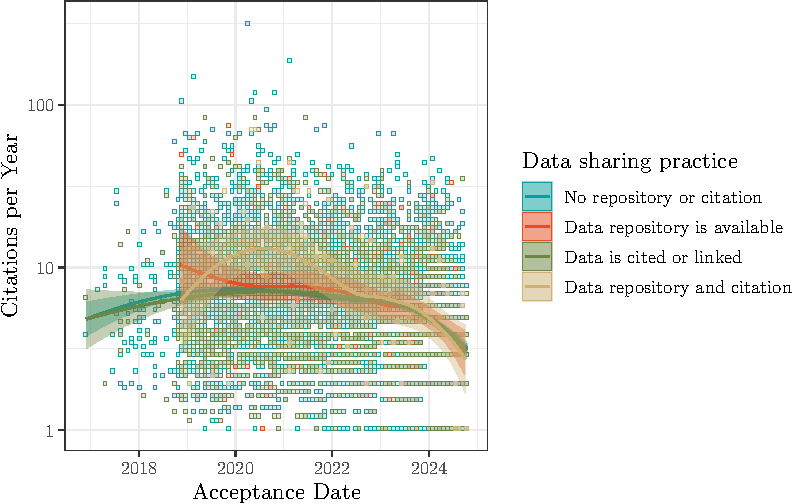
\includegraphics[keepaspectratio]{rrmeasures-paper_files/figure-pdf/fig-citations-1.pdf}}

}

\subcaption{\label{fig-citations-1}Citations per year by data sharing
practice.}

\centering{

\pandocbounded{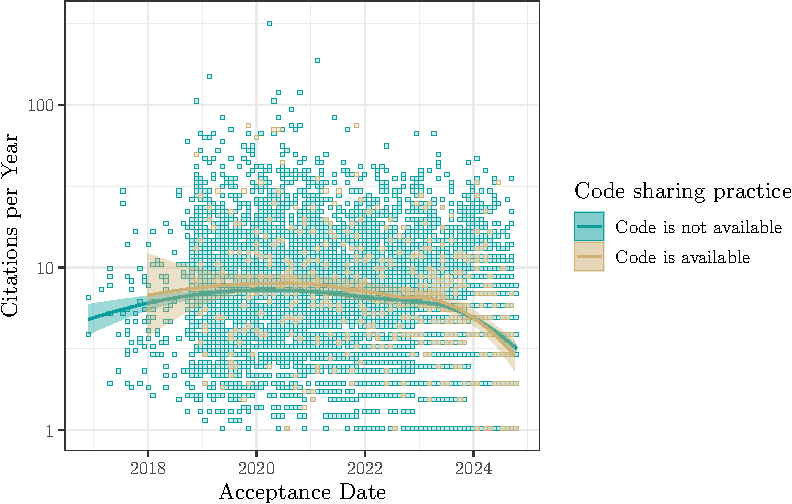
\includegraphics[keepaspectratio]{rrmeasures-paper_files/figure-pdf/fig-citations-2.pdf}}

}

\subcaption{\label{fig-citations-2}Citations per year by code sharing
practice.}

}

\caption{\label{fig-citations}Citations per year of each paper over time
by code and data-sharing practice, with a LOESS moving average line
applied for mean comparison.}

\end{figure}%

\begin{Shaded}
\begin{Highlighting}[]
\NormalTok{lm\_citations\_ctl }\OtherTok{\textless{}{-}} \FunctionTok{lm}\NormalTok{(}\FunctionTok{log}\NormalTok{(citations\_per\_year }\SpecialCharTok{+} \DecValTok{1}\NormalTok{) }\SpecialCharTok{\textasciitilde{}}\NormalTok{ journal }\SpecialCharTok{+}\NormalTok{ lda\_topic }\SpecialCharTok{+}\NormalTok{ region\_normalized, }\AttributeTok{data =}\NormalTok{ papers)}
\NormalTok{lm\_citations }\OtherTok{\textless{}{-}} \FunctionTok{update}\NormalTok{(lm\_citations\_ctl, . }\SpecialCharTok{\textasciitilde{}}\NormalTok{ . }\SpecialCharTok{+}\NormalTok{ is\_code\_available }\SpecialCharTok{+}\NormalTok{ data\_multi)}

\NormalTok{lm\_reviewtime\_ctl }\OtherTok{\textless{}{-}} \FunctionTok{update}\NormalTok{(lm\_citations\_ctl, }\FunctionTok{log}\NormalTok{(review\_time\_days }\SpecialCharTok{+} \DecValTok{1}\NormalTok{) }\SpecialCharTok{\textasciitilde{}}\NormalTok{ .)}
\NormalTok{lm\_reviewtime }\OtherTok{\textless{}{-}} \FunctionTok{update}\NormalTok{(lm\_citations, }\FunctionTok{log}\NormalTok{(review\_time\_days }\SpecialCharTok{+} \DecValTok{1}\NormalTok{) }\SpecialCharTok{\textasciitilde{}}\NormalTok{ .)}

\NormalTok{acitations }\OtherTok{\textless{}{-}} \FunctionTok{anova}\NormalTok{(lm\_citations\_ctl, lm\_citations)}
\NormalTok{areviewtime }\OtherTok{\textless{}{-}} \FunctionTok{anova}\NormalTok{(lm\_reviewtime\_ctl, lm\_reviewtime)}

\NormalTok{car}\SpecialCharTok{::}\FunctionTok{vif}\NormalTok{(lm\_citations)}
\end{Highlighting}
\end{Shaded}

\begin{verbatim}
                      GVIF Df GVIF^(1/(2*Df))
journal           7.644927  6        1.184717
lda_topic         8.023916 14        1.077208
region_normalized 1.262443  5        1.023579
is_code_available 1.766925  1        1.329257
data_multi        1.932137  3        1.116023
\end{verbatim}

\begin{Shaded}
\begin{Highlighting}[]
\NormalTok{cm }\OtherTok{\textless{}{-}} \FunctionTok{c}\NormalTok{(}
  \StringTok{"(Intercept)"} \OtherTok{=} \StringTok{"Intercept"}\NormalTok{,}
  \StringTok{"is\_code\_availableCode is available"} \OtherTok{=} \StringTok{"Code is available"}\NormalTok{,}
  \StringTok{"data\_multiData repository is available"} \OtherTok{=} \StringTok{"Data repository is available (NC, R)"}\NormalTok{,}
  \StringTok{"data\_multiData is cited or linked"} \OtherTok{=} \StringTok{"Data is cited or linked (C, NR)"}\NormalTok{,}
  \StringTok{"data\_multiData repository and citation"} \OtherTok{=} \StringTok{"Data repository and citation (C, R)"}\NormalTok{,}
  \StringTok{"journalTransportation Research Part A: Policy and Practice"} \OtherTok{=} \StringTok{"Journal: TR {-} A"}\NormalTok{,}
  \StringTok{"journalTransportation Research Part B: Methodological"} \OtherTok{=} \StringTok{"Journal: TR {-} B"}\NormalTok{,}
  \StringTok{"journalTransportation Research Part C: Emerging Technologies"} \OtherTok{=} \StringTok{"Journal: TR {-} C"}\NormalTok{,}
  \StringTok{"journalTransportation Research Part D: Transport and Environment"} \OtherTok{=} \StringTok{"Journal: TR {-} D"}\NormalTok{,}
  \StringTok{"journalTransportation Research Part E: Logistics and Transportation Review"} \OtherTok{=} \StringTok{"Journal: TR {-} E"}\NormalTok{,}
  \StringTok{"journalTransportation Research Part F: Traffic Psychology and Behaviour"} \OtherTok{=} \StringTok{"Journal: TR {-} F"}\NormalTok{,}

  \StringTok{"lda\_topicCOVID{-}19 Impact on Travel \& Activities"} \OtherTok{=} \StringTok{"Topic: COVID{-}19 Impact on Travel \& Activities"}\NormalTok{,}
  \StringTok{"lda\_topicSocial \& Policy Aspects of Mobility"} \OtherTok{=} \StringTok{"Topic: Social \& Policy Aspects of Mobility"}\NormalTok{,}
  \StringTok{"lda\_topicElectric Vehicles \& Ride{-}Sharing"} \OtherTok{=} \StringTok{"Topic: Electric Vehicles \& Ride{-}Sharing"}\NormalTok{,}
  \StringTok{"lda\_topicRoad Infrastructure \& Emergency Management"} \OtherTok{=} \StringTok{"Topic: Road Infrastructure \& Emergency Management"}\NormalTok{,}
  \StringTok{"region\_normalizedSouth America"} \OtherTok{=} \StringTok{"Region: South America"}
\NormalTok{)}

\FunctionTok{modelsummary}\NormalTok{(}
  \FunctionTok{list}\NormalTok{(}
    \StringTok{"Controls"} \OtherTok{=}\NormalTok{ lm\_reviewtime\_ctl, }
    \StringTok{"Open Science"} \OtherTok{=}\NormalTok{ lm\_reviewtime, }
    \StringTok{"Controls"} \OtherTok{=}\NormalTok{ lm\_citations\_ctl,}
    \StringTok{"Open Science"} \OtherTok{=}\NormalTok{ lm\_citations),}
  \AttributeTok{estimate =}\StringTok{"\{estimate\}\{stars\} "}\NormalTok{,}
  \AttributeTok{statistic =} \StringTok{"[\{conf.low\}, \{conf.high\}]"}\NormalTok{,}
  \AttributeTok{coef\_map =}\NormalTok{ cm,}
  \AttributeTok{gof\_omit =} \StringTok{"AIC|BIC|F"}\NormalTok{,}
  \AttributeTok{notes =} \FunctionTok{c}\NormalTok{(}\StringTok{"95\% confidence interval in parentheses"}\NormalTok{, }
  \StringTok{"Full controls: Journal, paper topic, and region of corresponding author."}\NormalTok{, }
  \StringTok{"Only significant controls displayed."}\NormalTok{),}
  \AttributeTok{format =} \StringTok{"tinytable"}
\NormalTok{)  }\SpecialCharTok{|\textgreater{}}
\NormalTok{  tinytable}\SpecialCharTok{::}\FunctionTok{group\_tt}\NormalTok{( }\AttributeTok{j =} \FunctionTok{list}\NormalTok{( }\StringTok{"Review time [days]"} \OtherTok{=} \DecValTok{2}\SpecialCharTok{:}\DecValTok{3}\NormalTok{, }\StringTok{"Citations per year"} \OtherTok{=} \DecValTok{4}\SpecialCharTok{:}\DecValTok{5}\NormalTok{))}
\end{Highlighting}
\end{Shaded}

\begin{table}

\caption{\label{tbl-incentives}Incentives for Open Science}

\centering{

\centering
\begin{talltblr}[         %% tabularray outer open
entry=none,label=none,
note{}={95\% confidence interval in parentheses},
note{ }={Full controls: Journal, paper topic, and region of corresponding author.},
note{  }={Only significant controls displayed.},
]                     %% tabularray outer close
{                     %% tabularray inner open
colspec={Q[]Q[]Q[]Q[]Q[]},
hline{2}={5}{solid, black, 0.03em},
hline{2}={2,4}{solid, black, 0.03em, l=-0.5},
hline{2}={3}{solid, black, 0.03em, r=-0.5},
hline{3}={1-5}{solid, black, 0.05em},
hline{35}={1-5}{solid, black, 0.05em},
hline{1}={1-5}{solid, black, 0.08em},
hline{40}={1-5}{solid, black, 0.08em},
column{3,5}={}{halign=c},
cell{1}{1}={}{halign=c},
cell{1}{2}={c=2}{halign=c},
cell{1}{4}={c=2}{halign=c},
cell{2-39}{1}={}{halign=l},
cell{2-39}{2}={}{halign=c},
cell{2-39}{4}={}{halign=c},
}                     %% tabularray inner close
& Review time [days] &  & Citations per year &  \\
& Controls & Open Science & Controls  & Open Science  \\
Intercept & \num{5.189}*** & \num{5.198}*** & \num{1.262}*** & \num{1.273}*** \\
& [\num{5.010}, \num{5.369}] & [\num{5.019}, \num{5.378}] & [\num{1.022}, \num{1.503}] & [\num{1.032}, \num{1.514}] \\
Code is available &  & \num{0.013} &  & \num{-0.067} \\
&  & [\num{-0.051}, \num{0.076}] &  & [\num{-0.154}, \num{0.020}] \\
Data repository is available (NC, R) &  & \num{-0.018} &  & \num{0.020} \\
&  & [\num{-0.099}, \num{0.064}] &  & [\num{-0.092}, \num{0.132}] \\
Data is cited or linked (C, NR) &  & \num{-0.019} &  & \num{-0.012} \\
&  & [\num{-0.045}, \num{0.007}] &  & [\num{-0.046}, \num{0.022}] \\
Data repository and citation (C, R) &  & \num{0.052} &  & \num{0.138}+ \\
&  & [\num{-0.068}, \num{0.171}] &  & [\num{-0.023}, \num{0.299}] \\
Journal: TR - A & \num{0.755}*** & \num{0.754}*** & \num{0.415}*** & \num{0.415}*** \\
& [\num{0.710}, \num{0.800}] & [\num{0.709}, \num{0.800}] & [\num{0.353}, \num{0.476}] & [\num{0.353}, \num{0.476}] \\
Journal: TR - B & \num{0.619}*** & \num{0.616}*** & \num{0.523}*** & \num{0.524}*** \\
& [\num{0.563}, \num{0.675}] & [\num{0.560}, \num{0.672}] & [\num{0.446}, \num{0.601}] & [\num{0.446}, \num{0.602}] \\
Journal: TR - C & \num{0.415}*** & \num{0.413}*** & \num{0.722}*** & \num{0.722}*** \\
& [\num{0.368}, \num{0.462}] & [\num{0.366}, \num{0.460}] & [\num{0.656}, \num{0.787}] & [\num{0.657}, \num{0.788}] \\
Journal: TR - D & \num{0.033} & \num{0.032} & \num{0.600}*** & \num{0.599}*** \\
& [\num{-0.017}, \num{0.083}] & [\num{-0.018}, \num{0.081}] & [\num{0.538}, \num{0.661}] & [\num{0.538}, \num{0.661}] \\
Journal: TR - E & \num{0.305}*** & \num{0.303}*** & \num{0.682}*** & \num{0.680}*** \\
& [\num{0.253}, \num{0.356}] & [\num{0.252}, \num{0.355}] & [\num{0.610}, \num{0.753}] & [\num{0.609}, \num{0.752}] \\
Journal: TR - F & \num{0.223}*** & \num{0.220}*** & \num{0.231}*** & \num{0.228}*** \\
& [\num{0.171}, \num{0.274}] & [\num{0.168}, \num{0.271}] & [\num{0.159}, \num{0.303}] & [\num{0.156}, \num{0.300}] \\
Topic: COVID-19 Impact on Travel \& Activities & \num{-0.213}** & \num{-0.213}** & \num{0.020} & \num{0.019} \\
& [\num{-0.347}, \num{-0.080}] & [\num{-0.347}, \num{-0.080}] & [\num{-0.160}, \num{0.200}] & [\num{-0.162}, \num{0.199}] \\
Topic: Social \& Policy Aspects of Mobility & \num{-0.097} & \num{-0.100} & \num{0.265}** & \num{0.262}** \\
& [\num{-0.225}, \num{0.030}] & [\num{-0.228}, \num{0.028}] & [\num{0.091}, \num{0.438}] & [\num{0.088}, \num{0.435}] \\
Topic: Electric Vehicles \& Ride-Sharing & \num{-0.035} & \num{-0.035} & \num{0.206}* & \num{0.208}* \\
& [\num{-0.170}, \num{0.100}] & [\num{-0.170}, \num{0.100}] & [\num{0.025}, \num{0.388}] & [\num{0.026}, \num{0.389}] \\
Topic: Road Infrastructure \& Emergency Management & \num{0.197}+ & \num{0.195}+ & \num{-0.270}* & \num{-0.271}* \\
& [\num{-0.019}, \num{0.412}] & [\num{-0.021}, \num{0.411}] & [\num{-0.537}, \num{-0.003}] & [\num{-0.538}, \num{-0.005}] \\
Region: South America & \num{0.047} & \num{0.044} & \num{-0.209}* & \num{-0.212}* \\
& [\num{-0.105}, \num{0.199}] & [\num{-0.108}, \num{0.197}] & [\num{-0.409}, \num{-0.009}] & [\num{-0.412}, \num{-0.013}] \\
Num.Obs. & \num{9185} & \num{9185} & \num{10480} & \num{10480} \\
R2 & \num{0.182} & \num{0.183} & \num{0.113} & \num{0.114} \\
R2 Adj. & \num{0.180} & \num{0.180} & \num{0.111} & \num{0.111} \\
Log.Lik. & \num{-7138.461} & \num{-7136.564} & \num{-11825.901} & \num{-11823.609} \\
RMSE & \num{0.53} & \num{0.53} & \num{0.75} & \num{0.75} \\
\end{talltblr}

}

\end{table}%

Table~\ref{tbl-incentives} presents estimates of log-linear regression
models of the review time in days and citations per year for the papers
in the dataset. These models include the journal, paper topic, and
region of corresponding author as dummy controls to account for
differing practices between journals and reviewers in topics.
Insignificant parameter estimates on these controls are suppressed in
Table~\ref{tbl-incentives} for clarity but the controls by themselves
explain virtually all of the reduction in variance in the models, with
insignificant reductions in the model \(F\)-statistic when markers for
data sharing and code availability are included (\(p\)-value of 0.44 for
review time and 0.33 for citations per year).

There are many considerations in this analysis, and in contemplating the
role of open science practices vis a vis researcher incentives. First,
researchers might not necessarily expect to see reduced review times
with open science practices. If a reviewer can follow and reproduce the
analysis in the paper during the review, this may result in more
thorough reviews and more extended resubmission processes. Improved and
more comprehensive reviews would benefit science, but would not
strengthen researcher incentives. Similarly, sharing data and code may
lead to more citations from others who pursue subsequent research, but
this effect is only likely if the original research question lends
itself to continued study, and if the code and data are packaged in such
a way that continued study is feasible. Further, the models presented in
Table~\ref{tbl-incentives} only explain one-tenth to one-fifth of the
variance in the data: important variables such as individual reviewer
availability, the complexity of the specific research question and
methods, and other sources of variance are not available to this
analysis but likely play a large role.


\bibliography{main.bib}



\end{document}
